

Измерение кривой дифракционного отражения в двухкристальной схеме представляет
собой измерение зависимости отраженного образцом рентгеновского излучения при
пошаговом повороте исследуемого кристалла относительно падающего на него
излучения в окрестности точного значения угла Брэгга.
Существует несколько схем измерения кривых отражения рентгеновского излучения.

\subsubsection*{$\omega$ - сканирование}
В данном типе сканирования кривая отражения измеряется путем поворота образца
относительно падающего пучка в плоскости дифракции. При таком сканировании
угол между падающим и дифрагированным пучками (угол рассеяния) остается постоянным
(рисунок ~\ref{ris:omega_scan}). Получаемая в результате кривая носит название кривой качания.


\begin{figure}[H]
  \centering
  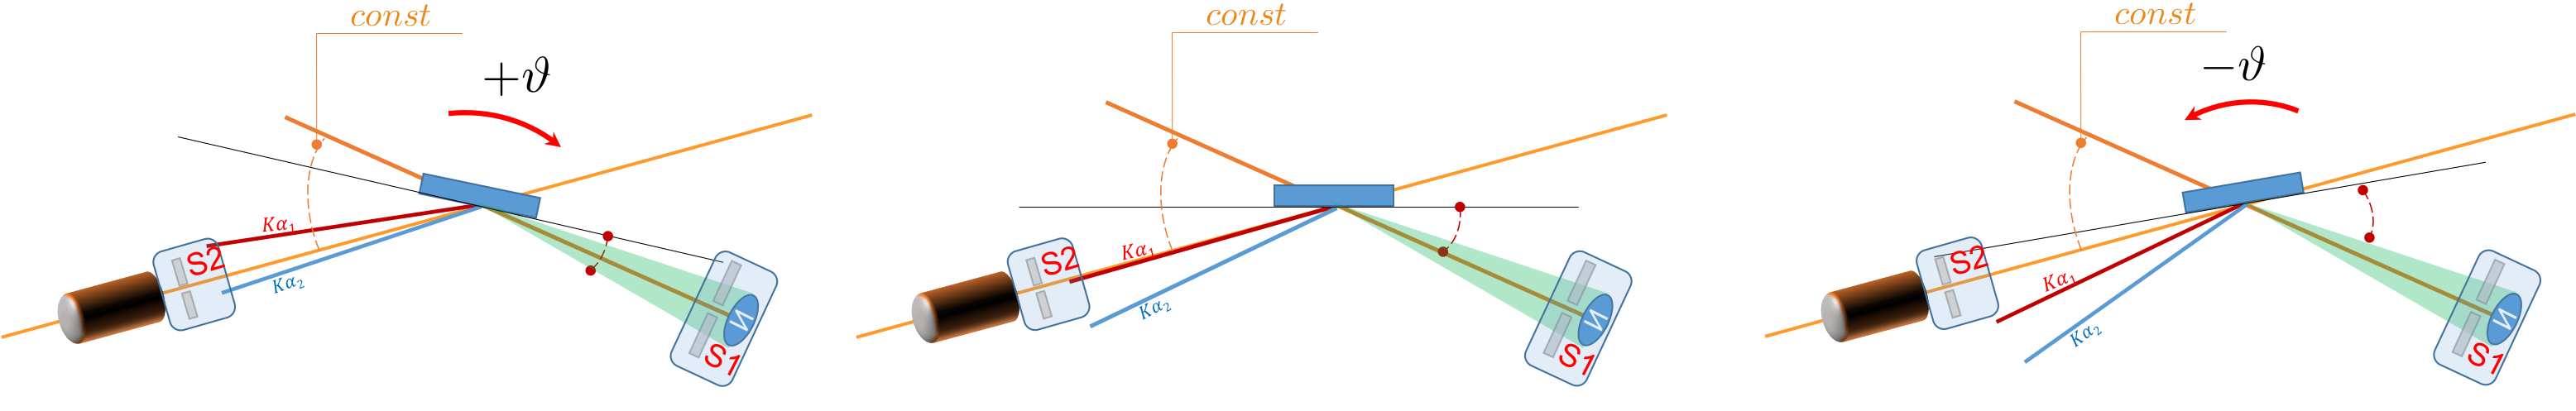
\includegraphics[width=1\textwidth]{images/omega_scan.png}
  \caption{Схема реализации $\omega $ - сканирования}
  \label{ris:omega_scan}
\end{figure}

\subsubsection*{$\vartheta - 2\vartheta$ - сканирование}
В отличие от предыдущего, данный метод сканирования соответствует изменению
 модуля вектора рассеяния при неизменном его угловом положении
 (рисунок ~\ref{ris:theta_2theta_scan}). Угловое положение падающего пучка и
 детектора изменяется синхронно и симметрично относительно используемой системы
 атомных плоскостей, а установленная перед детектором апертурная щель вырезает
  только зеркально отраженную часть пучка. Именно поэтому при построении карт
   пространственного распределения спектра полосы щелей на этих картах остаются
   неподвижными (т.к. несмотря на движение щели  $S_2$ в процессе
    $\vartheta - 2\vartheta$ -  сканирования ее отстройка от зеркального
    положения всегда равна 0).

 \begin{figure}[H]
   \centering
   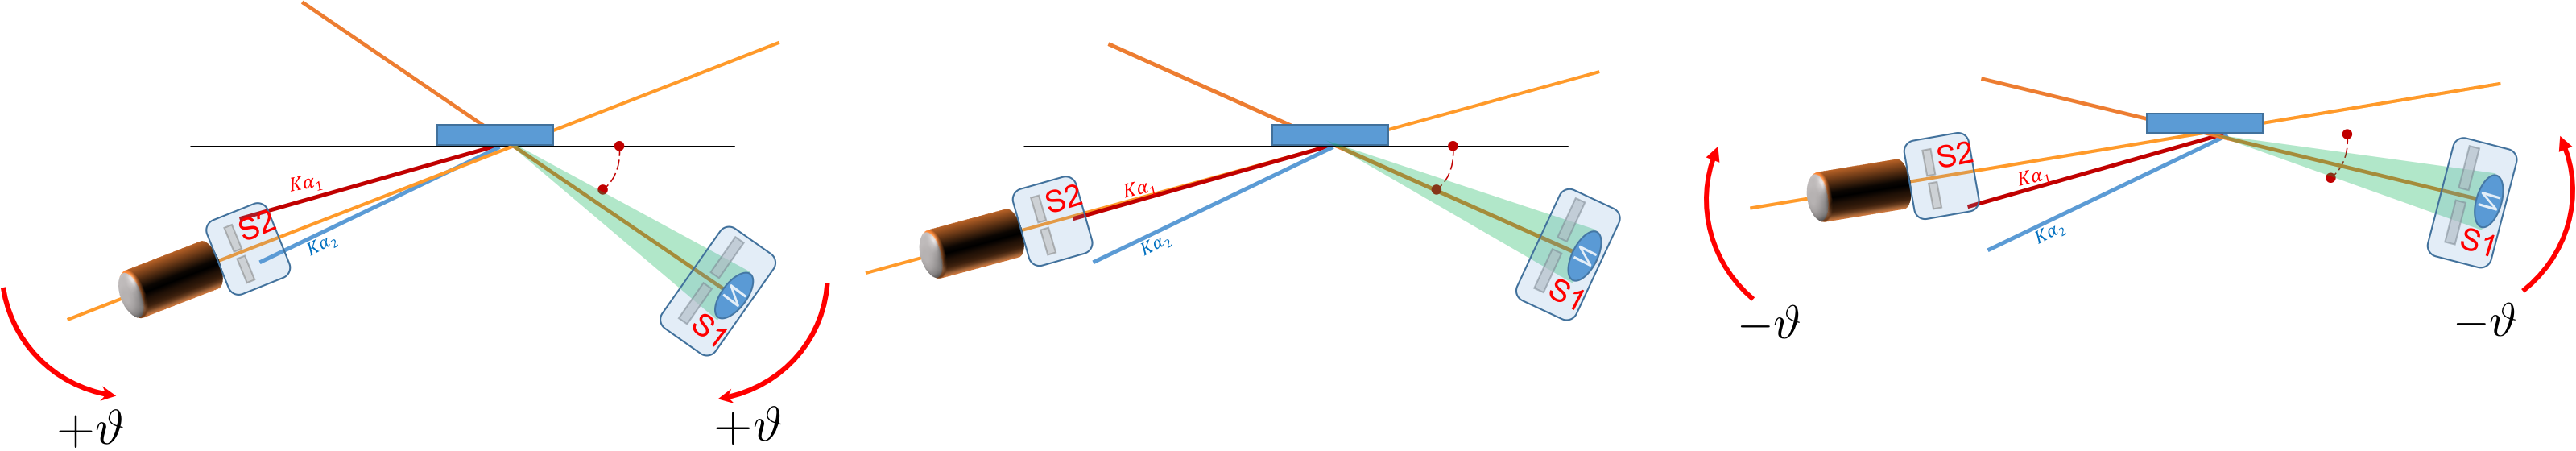
\includegraphics[width=1\textwidth]{images/theta_2theta_scan.png}
   \caption{Схема реализации $\vartheta - 2\vartheta$ - сканирования}
   \label{ris:theta_2theta_scan}
 \end{figure}
Кроме того, используемый подход позволяет наглядно продемонстрировать интересный эффект.
 Независимо от ширины входной и приемной щелей характеристическая линия спектра
 трубки $k_{\alpha 2}$ всегда вносит вклад в КДО, проявляясь в виде дополнительного
 пика на ее хвосте (рис. 2.21). Данный слабый пик возникает за счет того, что
 даже при очень малой входной щели $S_1$ линия $k_{\alpha 2}$ будет, отражаясь на «хвосте»
 кривой монохроматора, пролетать через входную щель и, при определённом угле
 поворота образца, интенсивно дифрагировать в максимуме его собственной кривой
 отражения и давать весомый ($~10^{-6}$) вклад в общую интенсивность КДО.
